\begin{center}
	\vspace{0.5cm}
	{\parbox{16cm}
		{\small{\centering{\textbf{Аннотация}\\
					\hspace{0.6cm} 
					В этом отчёте изложены результаты выполнения лабораторной работы «ЯМР-релаксация». Были проделаны измерения времени продольной и поперечной релаксации протонной намагниченности для воды и растворов $MnSO_4$ и $Na_2 SO_4$ различной концентрации. Полученные времена релаксации. Работа выполнялась с использованием ЯМР-релаксометра \textit{Bruker Minispec}.
				}
			}
		}
	}
\end{center}

\textbf{\emph{Цель работы:}}
изучить механизм релаксации ядерной намагниченности и освоить методы измерения продольной и поперечной релаксации протонов.
\section{Теоретическое введение}
\subsection{Суть ЯМР}
Явление ЯМР заключается в резонансном поглощении электромагнитной энергии макроскопической системой ядерных магнитных моментов, помещенных в постоянное внешнее магнитное поле. Ядерные магнитные моменты связаны с наличием у протонов и нейтронов \textit{спинов}.

Энергия $E$ магнитного момента, находящегося в постоянном магнитном поле $\vec{B_0}$, равна
\begin{equation}
\label{E_in_field}
E = - (\vec{\mu}, \vec{B_0}) = -\mu B_0 \cos \theta = - g \beta_N B_0 m_z
\end{equation}
где $\theta$ -- угол между направлениями векторов $\mu$ и $B_0$, а $ m_z $ -- проекция спина на ось $z$, совпадающую с направлением $ B_0 $, $\beta_N = 5.0508 \cdot 10^{-27} \text{Дж}/\text{Тл}$ -- ядерный магнетон, $g$ -- так называемый фактор Ланде, представляющий из себя безразмерную величину (индивидуален для каждого вещества).
Протон имеет спин $ I = 1/2 $, поэтому возможные значения проекции спина на ось квантования равны $ m_z = \pm 1/2 $.

Из (\ref{E_in_field}) следует, что в магнитном поле $B_0$ происходит расщепление на два состояния, имеющие разную энергию.
Между этими уровнями возможны переходы при поглощении кванта электромагнитной энергии определенной частоты -- это и есть суть ЯМР.

\subsection{Уравнение Блоха и радиочастотные импульсы}
В равновесном состоянии суммарная намагниченность $M$ ансамбля спинов, помещенных во внешнее постоянное магнитное поле, ориентируется параллельно направлению приложенного поля. Удобной моделью для описания поведения вектора суммарной намагниченности в магнитном поле является феноменологическая теория Блоха.
\begin{equation}
\label{Bloh_simple}
\dfrac{d \vec{M}(t)}{dt} = \gamma \vec{M}(t) \times \vec{B}(t)
\end{equation}
где $\gamma = \dfrac{2 \pi g \beta_N}{h}$.

При воздействии радиочастотного поля $ \vec{B}_1(t) = \vec{B}_{1m} \sin(\omega t) $, направленного перпендикулярно направлению постоянного магнитного поля $ B_0 $, на систему спинов намагниченность последней будет находиться под воздействием поля $\vec{B}(t) = \vec{B}_1 (t) + \vec{B}_0$.
Действие переменного поля удобно анализировать на основе уравнения Блоха, используя систему координат, вращающуюся с Ларморовой частотой $ \omega_0 = \gamma B_0 $ вокруг направления $z$ постоянного поля. В этой системе уравнение (\ref{Bloh_simple}) без учета релаксации имеет вид:
\begin{equation}
\label{Bloh_rotation}
\dfrac{d \vec{M}(t)}{dt} = \gamma \vec{M}(t) \times \left(\vec{B}(t) - \dfrac{\omega_0}{\gamma} \right)
\end{equation}
Под действием переменного электромагнитного поля с резонансной частотой $ \omega_0 = \gamma B $ вектор намагниченности во вращающейся СК совершает прецессию вокруг вектора $B_1$ поля с угловой частотой $ \omega_1 = \gamma B_1 $. Если переменное магнитное поле действует в течение короткого времени $ \tau_\theta $, то вектор намагниченности повернется на угол:
\begin{equation}
\label{Theta_def}
\theta = \gamma B_1 \tau_\theta
\end{equation}
где $ \theta $ -- угол поворота в радианах, $ \gamma  $ -- гиромагнитное отношение (для ядер $^1$H $ \gamma = 26.75~\cdot~10^7 \text{рад }\text{с}^{-1}\text{Тл}^{-1} $)

Для поворота суммарной намагниченности на заданный угол $\theta$ настраивают амплитуду $ B_1 $ и длительность $ \tau_\theta $ в соответствии с (\ref{Theta_def}). При этом для угла $90 ^{\circ}$ импульс называется \textit{$\pi /2$-импульсом}, а для угла $180 ^{\circ}$ называется \textit{$ \pi $-импульсом}.

\begin{figure}[h]
	\centering
	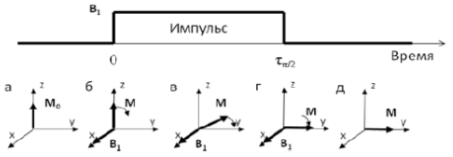
\includegraphics[width=0.7\linewidth]{M-rotation}
	\caption{Поведение суммарной намагниченности под действием $\pi /2$-импульса (вращающаяся СК). \textbf{а} -- до включения; \textbf{б} -- начало действия импульса; \textbf{в} -- поворот намагниченности; \textbf{г} --  окончание действия импульса; \textbf{д} -- прецессия намагниченности вокруг оси $z$ после выключения импульса}
	\label{fig:m-rotation}
\end{figure}


\subsection{Релаксация ядерной намагниченности}
Процесс восстановления суммарной намагниченности к исходному равновесному состоянию называют \textit{релаксацией намагниченности}. Уравнение Блоха с учетом процессов релаксации выглядит следующим образом
\begin{align}
\label{Bloh-relaxaion}
\dfrac{d M_x}{dt} &= \gamma \left[ M_y B_z - M_z B_y\right] - \dfrac{M_x}{T_2} \\
\dfrac{d M_y}{dt} &= \gamma \left[ M_z B_x - M_x B_z\right] - \dfrac{M_y}{T_2} \\
\dfrac{d M_z}{dt} &= \gamma \left[ M_x B_y - M_y B_x\right] - \dfrac{M_z - M_0}{T_1} \\
\end{align}

Решение уравнения Блоха после окончания действия $\pi /2$-импульса выглядит следующим образом:
\begin{align}
	\vec{M}(t) = M_0
	\begin{pmatrix}
		0 \\
		e^{-t/T_2} \\
		1 - e^{-t/T_1}
	\end{pmatrix}
\end{align}

\subsection{Механизмы ЯМР-релаксации}